\documentclass[border=6pt]{standalone}
\usepackage{tikz}
\usepackage[edges]{forest}
\usetikzlibrary{arrows.meta,positioning,calc,decorations.pathreplacing,shapes.geometric}
\begin{document}
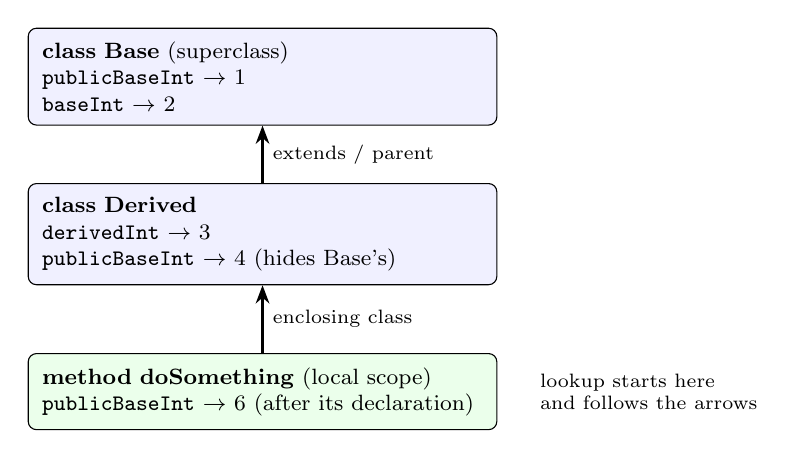
\begin{tikzpicture}[>=Stealth,font=\small,
  tbl/.style={draw,rounded corners=3pt,fill=blue!6,align=left,inner sep=5pt,font=\footnotesize,text width=5.6cm}]
\node[tbl] (B) at (0,0) {\textbf{class Base} (superclass)\\ \texttt{publicBaseInt} $\to$ 1\\ \texttt{baseInt} $\to$ 2};
\node[tbl] (D) at (0,-2.0) {\textbf{class Derived}\\ \texttt{derivedInt} $\to$ 3\\ \texttt{publicBaseInt} $\to$ 4 (hides Base's)};
\node[tbl,fill=green!8] (M) at (0,-4.0) {\textbf{method doSomething} (local scope)\\ \texttt{publicBaseInt} $\to$ 6 (after its declaration)};
\draw[->,thick] (D) -- node[right,font=\scriptsize]{extends / parent} (B);
\draw[->,thick] (M) -- node[right,font=\scriptsize]{enclosing class} (D);
\node[font=\scriptsize,anchor=west,align=left] at (3.4,-4.0) {lookup starts here\\and follows the arrows};
\end{tikzpicture}
\end{document}
